\documentclass[xcolor=dvipsnames, aspectratio=169, 10pt]{beamer}

\usepackage{import}

\import{../../template}{main.tex}
\newcommand{\Title}{Logic}
\newcommand{\Logo}{example-image-c}
\addbibresource{refs.bib}
\usepackage{tikz}
\usetikzlibrary {automata,positioning, calc}


\begin{document}
\TitlePage
\SectionPage
\SubsectionPage
\ProgressBar
\PageNumbering
\section{Introduction}
\begin{frame}
	Principal tasks of proof theory \cite{buss1998handbook}
	\begin{enumerate}
		\item to formulate systems of logic and sets of axioms which are appropriate for formalizing mathematical proofs and to characterize what results follow from certain axioms;
		\item to study the structure of formal proofs (normal forms, syntactic facts);
		\item to study additional information can be extracted from proofs beyond the truth of the theorem being proved (computational or constructive information);
		\item to study how best to construct formal proofs by a computer.
	\end{enumerate}
\end{frame}

\begin{frame}
	Bye
\end{frame}
\section{Propositional Logic}
\subsection{Compactness Theorem}
\begin{frame}
  Test
  \cite{buss1998handbook}
  \begin{enumerate}
    \item asdasd $\dfrac{a}{B}$
    \item asdasdasdasd
    \item asdasd
  \end{enumerate}
  \begin{figure}
    \centering
    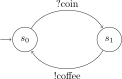
\includegraphics{images/tikz_1.svg}
    \caption{LTSs for vending machines}
    \label{fig:lts-vending-machines}
  \end{figure}
\end{frame}
\begin{frame}
  \printbibliography
\end{frame}
\end{document}
